\documentclass{article}%
\usepackage[T1]{fontenc}%
\usepackage[utf8]{inputenc}%
\usepackage{lmodern}%
\usepackage{textcomp}%
\usepackage{lastpage}%
\usepackage[tmargin=1cm,lmargin=1cm]{geometry}%
\usepackage{graphicx}%
%
%
%
\begin{document}%
\normalsize%
\section{Sinewave Generator}%
\label{sec:Sinewave Generator}%


\begin{figure}[h!]%
\centering%
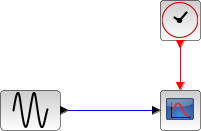
\includegraphics[width=120px]{/home/kyoya2212/Test_files/sinewave_generator.png}%
\caption{SineWave Generator}%
\end{figure}

%
\subsection{GenSin}%
\label{subsec:GenSin}%
\begin{tabular}{|c|c|}%
\hline%
Name&Value\\%
\hline%
magnitude&1\\%
\hline%
frequency&1\\%
\hline%
pulse&0\\%
\hline%
\end{tabular}

%
\subsection{Cscope}%
\label{subsec:Cscope}%
\begin{tabular}{|c|c|}%
\hline%
Name&Value\\%
\hline%
Color Vector&1 3 5 7 9 11 13 15\\%
\hline%
Output window number&{-}1\\%
\hline%
Output window position&{[}{]}\\%
\hline%
Output window sizes&{[}600;400{]}\\%
\hline%
Ymin&{-}15\\%
\hline%
Ymax&15\\%
\hline%
Refresh period&30\\%
\hline%
Buffer Size&20\\%
\hline%
Accept Herited Events&0\\%
\hline%
Name of Scope&\\%
\hline%
\end{tabular}

%
\subsection{Clock}%
\label{subsec:Clock}%
\begin{tabular}{|c|c|}%
\hline%
Name&Value\\%
\hline%
Period&0.1\\%
\hline%
Initialisation Time&0.1\\%
\hline%
\end{tabular}

%
\end{document}